\documentclass[final]{beamer}

\usepackage[scale=1.24]{beamerposter} % Use the beamerposter package for laying out the poster

\usetheme{confposter} % Use the confposter theme supplied with this template

\setbeamercolor{block title}{fg=nblue,bg=white} % Colors of the block titles
\setbeamercolor{block body}{fg=black,bg=white} % Colors of the body of blocks
\setbeamercolor{block alerted title}{fg=white,bg=dblue!70} % Colors of the highlighted block titles
\setbeamercolor{block alerted body}{fg=black,bg=dblue!10} % Colors of the body of highlighted blocks
% Many more colors are available for use in beamerthemeconfposter.sty

\newlength{\sepwid}
\newlength{\onecolwid}
\setlength{\paperwidth}{48in} % A0 width: 46.8in
\setlength{\paperheight}{36in} % A0 height: 33.1in
\setlength{\sepwid}{0.024\paperwidth} % Separation width (white space) between columns
\setlength{\onecolwid}{0.301\paperwidth} % Width of one column
\setlength{\topmargin}{-0.5in} % Reduce the top margin size
% -----------------------------------------------------------

\usepackage{graphicx}  % Required for including images

\usepackage{booktabs} % Top and bottom rules for tables

% ----------------------------------------------------------------------------------------
%	TITLE SECTION
% ----------------------------------------------------------------------------------------

\def\realtitle{Association of single ultracold molecules in optical tweezers}

\title{%
  \texorpdfstring{%
    \makebox[\linewidth]{%
      \makebox[0pt][l]{%
        \raisebox{\dimexpr-\height+\baselineskip}[0pt][0pt]
        {
\includegraphics[height=4\baselineskip]{harvard}}% Left logo
      }\hfill
      \makebox[0pt]{\textcolor{dblue}{\realtitle}}%
      \hfill\makebox[0pt][r]{%
        \raisebox{\dimexpr-\height+0.5\baselineskip}[0pt][0pt]
        {
\includegraphics[height=3\baselineskip]{cua}}% Right logo
      }%
    }%
  }
  {\realtitle}} % Poster title

\author{Yichao Yu, Jonathan Hood, Lee R. Liu, Jessie T. Zhang, Yen-Wei Lin,
  Kenneth Wang, Rem\'y Vatr\'e, Till Rosenband, Kang-Kuen Ni}
\institute{Harvard-MIT Center for Ultracold Atoms\\
  Department of Chemistry and Chemical Biology and Department of Physics, Harvard University}

% ----------------------------------------------------------------------------------------

\begin{document}

\addtobeamertemplate{block end}{}{\vspace*{2ex}} % White space under blocks
\addtobeamertemplate{block alerted end}{}{\vspace*{2ex}} % White space under highlighted (alert) blocks

\setlength{\belowcaptionskip}{2ex} % White space under figures
\setlength\belowdisplayshortskip{2ex} % White space under equations

\begin{frame}[t] % The whole poster is enclosed in one beamer frame

  \begin{columns}[t] % The whole poster consists of three major columns, the second of which is split into two columns twice - the [t] option aligns each column's content to the top

    \begin{column}{\sepwid}\end{column} % Empty spacer column

    \begin{column}{\onecolwid} % The first column

      % ----------------------------------------------------------------------------------------
      %	QUICK REVISION
      % ----------------------------------------------------------------------------------------

      \begin{block}{Quick Revision}

        \textbf{Forms of Quadratic Function}
        \begin{itemize}
        \item $f(x) = ax^2+bx+c$ is called the \textbf{standard form}.
        \item $f(x) = a(x-x_1)(x-x_2)$ is called the \textbf{factored form}, where $x_1$ and $x_2$ are the roots of the quadratic function.
        \item $f(x) = a(x-h)^2+k$ is called the \textbf{vertex form}.
        \end{itemize}

        \textbf{Delta $\Delta$}\\*
        $\Delta$ determines tells us how many solutions quadratic equation have:
        $$\text{number of solutions}=
        \begin{cases}
          2 &\text{when } \Delta > 0\\
          1 &\text{when } \Delta = 0\\
          0 &\text{when } \Delta < 0
        \end{cases}
        $$


        \textbf{The Quadratic Formula}
        $$x = \frac{-b\pm \sqrt{\Delta}}{2a}$$

        \textbf{Graph of Quadratic Function}

      \end{block}

      % ------------------------------------------------

      \begin{figure}
        % 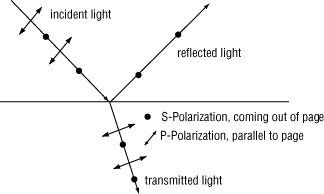
\includegraphics[width=0.8\linewidth]{1.jpg}
        \caption{Graph of $f(x)=ax^2|_{\{0.1, 0.3, 1.0, 3.0\}}$}
      \end{figure}

      % ----------------------------------------------------------------------------------------

    \end{column} % End of the first column

    \begin{column}{\sepwid}\end{column} % Empty spacer column

    \begin{column}{\onecolwid} % Begin a column which is two columns wide (column 2)

      \begin{columns}[t,totalwidth=\onecolwid] % Split up the two columns wide column

        \begin{column}{0.5\onecolwid}\vspace{-.6in} % The first column within column 2 (column 2.1)

          % ----------------------------------------------------------------------------------------
          %	MATERIALS
          % ----------------------------------------------------------------------------------------

          \begin{block}{Factorising a Quadratic}

            Factorising a quadratic means putting it into two brackets, and is useful if you're trying to draw a graph of a quadratic solve a quadratic equation. It's pretty easy if $a=1$ (in $ax^2+bx+c$ form), but can be a real pain otherwise.
            \newline
            \newline
            In order to factorise a quadratic you should follow steps outlined below:

            \begin{enumerate}
            \item Rearrange the equation into the standard $ax^2+bx+c$ form.
            \item Write down two brackets: $(x\ \ \ )(x\ \ \ )$
            \item Find two numbers that multiply to give 'c' and add or subtract to give 'b' (ignoring signs).
            \item Put the numbers in brackets and choose their signs.
            \end{enumerate}

          \end{block}

          % ----------------------------------------------------------------------------------------

        \end{column} % End of column 2.1

        \begin{column}{0.5\onecolwid}\vspace{-.6in} % The second column within column 2 (column 2.2)

          % ----------------------------------------------------------------------------------------
          %	P
          % ----------------------------------------------------------------------------------------

          \begin{block}{Factorising- Tasks}
            1. Factorise $x^2-x-12$.
            2. Solve $x^2-8=2x$ by factorising.

          \end{block}

          % ----------------------------------------------------------------------------------------

        \end{column} % End of column 2.2

      \end{columns} % End of the split of column 2 - any content after this will now take up 2 columns width

      % ----------------------------------------------------------------------------------------
      %	IMPORTANT To REMEMBER
      % ----------------------------------------------------------------------------------------

      \begin{alertblock}{Myth of Delta $\Delta$}

        It's commonly believed that in order to work out roots of a quadratic function you must count $\Delta$ and use other previously established formulas. However this is untrue since factorising in many cases is as good or even better than simply counting $\Delta$.

      \end{alertblock}

    \end{column} % End of the second column

    \begin{column}{\sepwid}\end{column} % Empty spacer column

    \begin{column}{\onecolwid} % The third column

      % ----------------------------------------------------------------------------------------
      %	CONCLUSION
      % ----------------------------------------------------------------------------------------

      \begin{block}{Vieta's Formulas- Task}
        1. Prove that $$x_1x_2 = \frac{c}{a}$$
        \[\]
        \[\]
        \[\]
        \[\]
        \[\]

      \end{block}


      % ----------------------------------------------------------------------------------------
      %	ACKNOWLEDGEMENTS
      % ----------------------------------------------------------------------------------------

      \setbeamercolor{block title}{fg=red,bg=white} % Change the block title color

      \begin{block}{Glossary}

        \begin{table}
          \vspace{2ex}
          \begin{tabular}{l l l l}
            \toprule
            \textbf{verb} & \textbf{noun} & \textbf{meaning}\\
            \midrule
            add & addition & $+$ \\
            subtract & subtraction & $-$ \\
            multiply & multiplication & $\cdot$ \\
            divide & division & $\div$ \\
            solve & solution & getting answer \\
            substitute & substitution & $t=x^2$ \\



            \bottomrule
          \end{tabular}
          \caption{Word Formation}
        \end{table}


      \end{block}

      \setbeamercolor{block alerted title}{fg=black,bg=norange} % Change the alert block title colors
      \setbeamercolor{block alerted body}{fg=black,bg=white} % Change the alert block body colors

      \begin{alertblock}{Some Necessary and Useful Vocabulary}

        \begin{itemize}
        \item (n.) sign $\rightarrow$ $+$ or $-$
        \item (n.) equation $\rightarrow something = 0$
        \item (n.) factor $\rightarrow$ two multiplied factors give result
        \item (v.) factorise $\rightarrow$ putting into brackets
        \item (n.) coefficient $\rightarrow$ a constant number i.e. $a$, $b$, $c$ in a pattern $ax^2+bx+c$
        \item (n.) quadratic function $\rightarrow$ $f(x) = ax^2+bx+c$
        \item (n.) root $\rightarrow$ $\sqrt{sth}$ or solution of quadratic equation
        \item (n.) formula $=$ pattern
        \end{itemize}

      \end{alertblock}


      % ----------------------------------------------------------------------------------------

    \end{column} % End of the third column

  \end{columns} % End of all the columns in the poster

\end{frame} % End of the enclosing frame

\end{document}
